\documentclass{beamer}

\usepackage[utf8]{inputenc}
\usepackage[T1]{fontenc}
\usepackage{graphicx}
\usepackage{subfig}
\usepackage[french]{babel}

\usetheme{Warsaw}

\title{Displacement mapping shader}
\subtitle{Per-pixel displacement mapping with distance functions}
\author[K.~Bannier, C.~Delambily, N.~Laboureur, A.~Louarn]{Kévin Bannier \and Clémentine Delambily \\ Nicolas Laboureur \and Amaury Louarn}
\institute{%
    Parcours Imagerie Numérique\\
    École supérieure d'ingénieurs de Rennes 1\\
    Université de Rennes 1
}
\date{15 Janvier 2016}

\AtBeginSection{%
    \begin{frame}
        \frametitle{Sommaire}
        \tableofcontents[currentsection]
    \end{frame}
}

\begin{document}
\frame{\titlepage}

\section{Introduction}
\subsection{Concept}
\begin{frame}
    \frametitle{Présentation}
    \begin{itemize}
        \item Ajouter des détails à un mesh
        \item Modification de la position perçue des pixels
    \end{itemize}
    \begin{center}
        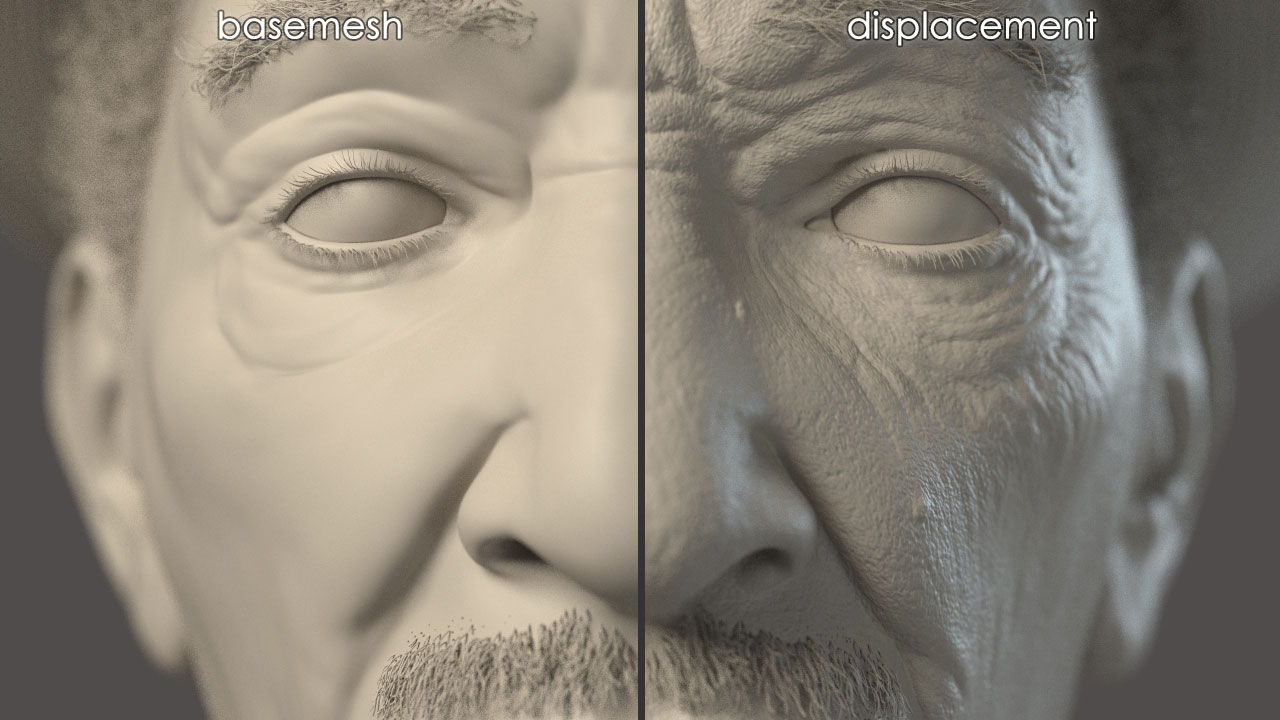
\includegraphics[width=0.9\textwidth]{images/mesh_vs_displacement}
    \end{center}
\end{frame}
\subsection{Différence avec le bump mapping}
\begin{frame}
    \frametitle{Différence avec le bump mapping}
    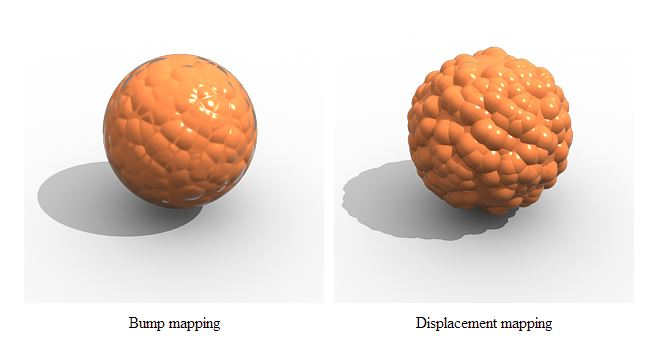
\includegraphics[width=\textwidth]{images/bump_vs_displacement}
\end{frame}
\subsection{Implémentations}
\begin{frame}
    \frametitle{Différentes manières}
    \begin{itemize}
        \item Tesselation
            \begin{itemize}
                \item Déplacement \og{}physique \fg{}
                \item Ajout de vertex dans un mesh
                \item Implémentation inégale
                    \begin{itemize}
                        \item DirectX $\geq 11$
                        \item OpenGL $\geq 4$
                        \item Indisponible pour webGL
                    \end{itemize}
            \end{itemize}
        \item \emph{Ray tracing} avec fonctions distances
            \begin{itemize}
                \item Déplacement \og{}virtuel \fg{}
            \end{itemize}
    \end{itemize}
\end{frame}
\begin{frame}
    \frametitle{Displacement mapping avec tessellation}
    \begin{columns}[t]
        \begin{column}{0.5\textwidth}
            \centering
            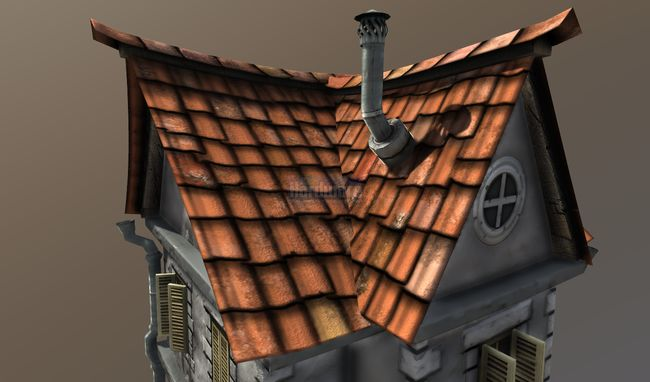
\includegraphics[width=0.9\textwidth]{images/tesselation_off}\\
            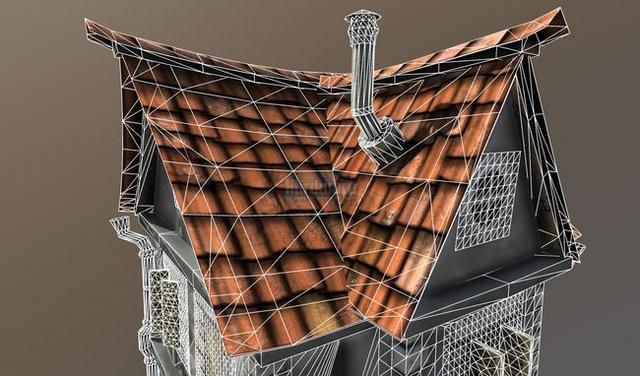
\includegraphics[width=0.9\textwidth]{images/tesselation_off_mesh}\\
            Tessellation on
        \end{column}
        \begin{column}{0.5\textwidth}
            \centering
            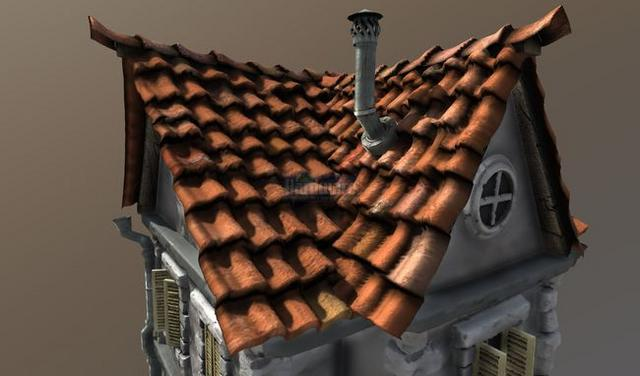
\includegraphics[width=0.9\textwidth]{images/tesselation_on}\\
            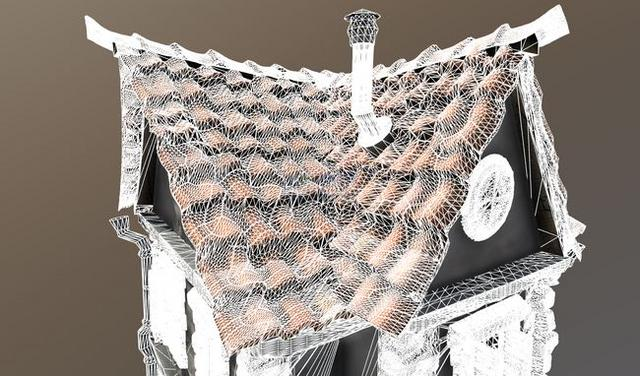
\includegraphics[width=0.9\textwidth]{images/tesselation_on_mesh}\\
            Tessellation off
        \end{column}
    \end{columns}
\end{frame}

\section{Fonctionnement}
\subsection{Carte des distances}
\begin{frame}
    \frametitle{Carte des distances}
    \begin{itemize}
        \item Transformation d'une carte des hauteurs 2D (\emph{heightmap}) en carte de distances en 3 dimensions (\emph{distance map})
    \end{itemize}
    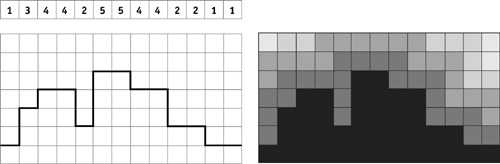
\includegraphics[width=\textwidth]{images/sample_distancemap}
\end{frame}
\subsection{Ray marching}
\begin{frame}
    \frametitle{Ray marching}
    \begin{itemize}
        \item Suivi du parcours d'un rayon
        \item Parcours depuis la surface du triangle
        \item Parcours pas-à-pas grâce à la \emph{distance map}
    \end{itemize}
\end{frame}
\begin{frame}
    \frametitle{Ray marching~: exemple}
    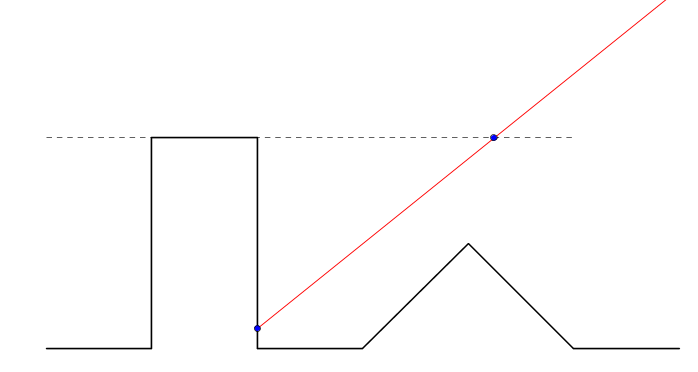
\includegraphics[width=\textwidth]{images/rayTracing-0}
\end{frame}
\begin{frame}
    \frametitle{Ray marching~: exemple}
    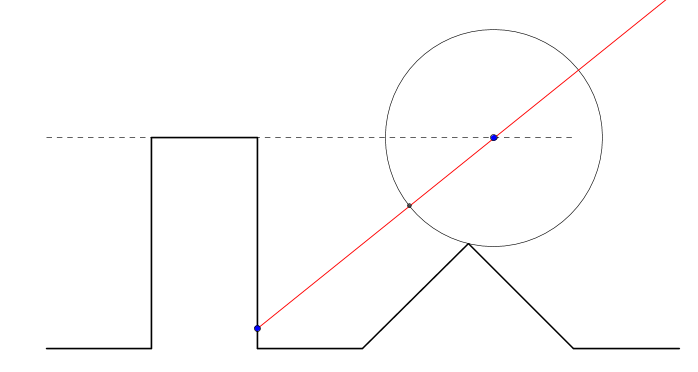
\includegraphics[width=\textwidth]{images/rayTracing-1}
\end{frame}
\begin{frame}
    \frametitle{Ray marching~: exemple}
    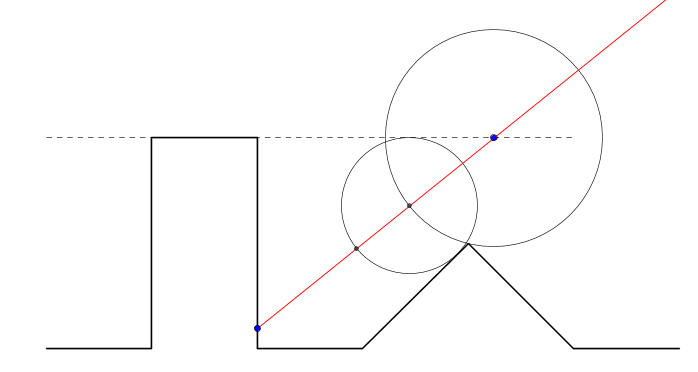
\includegraphics[width=\textwidth]{images/rayTracing-2}
\end{frame}
\begin{frame}
    \frametitle{Ray marching~: exemple}
    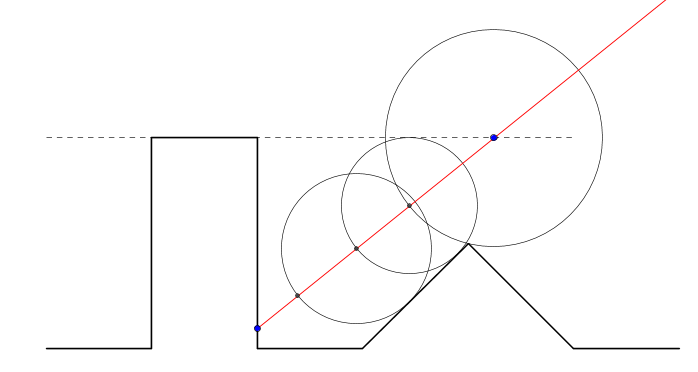
\includegraphics[width=\textwidth]{images/rayTracing-3}
\end{frame}
\begin{frame}
    \frametitle{Ray marching~: exemple}
    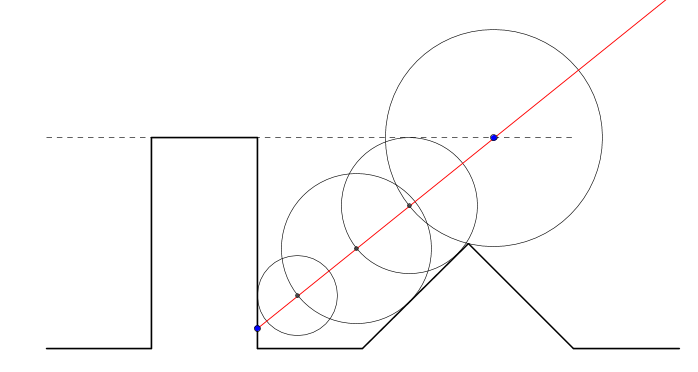
\includegraphics[width=\textwidth]{images/rayTracing-4}
\end{frame}
\begin{frame}
    \frametitle{Ray marching~: exemple}
    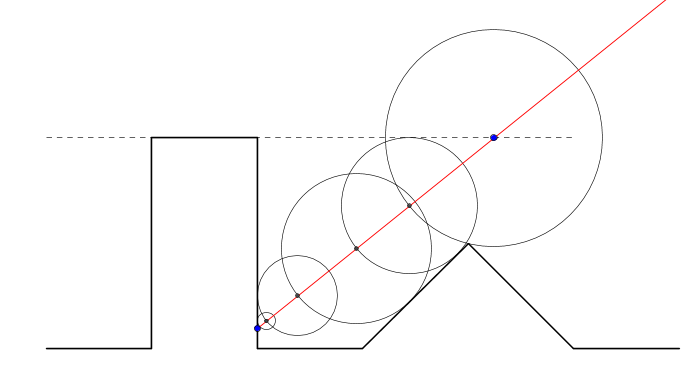
\includegraphics[width=\textwidth]{images/rayTracing-5}
\end{frame}

\section{Application}
\subsection{Problèmes rencontrés}
\begin{frame}
    \frametitle{Problèmes rencontrés}
    \begin{itemize}
        \item Pas de prise en charge des textures 3D sous webGL
        \item atomicGL pas adapté pour gérer des tableaux de textures 2D
        \item Limitation du nombre d'appels à \texttt{texture2D} par fragment shader
    \end{itemize}
\end{frame}
\subsection{Résultats}
\begin{frame}
    \frametitle{Résultats}
    \centering
    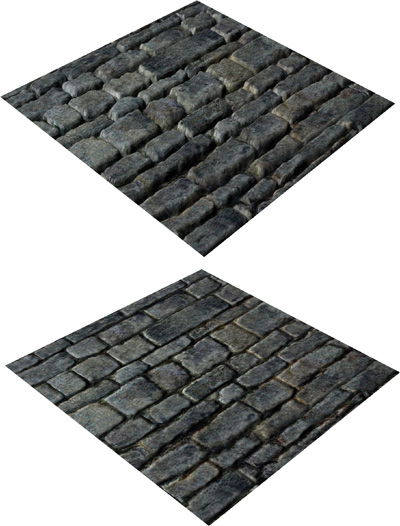
\includegraphics[scale=0.5]{images/displaced_stone}
\end{frame}

\end{document}
